\chapter{Literature review}
\label{literaturereview}

 \lhead{\emph{Literature Review}} % Chapter title for thesis template 

\section{Search strategy}
\label{searchstrategy}

In order to identify an appropriate set of key search terms for the literature review, a population, intervention, comparison and outcome (PICO) framework was utilised (\autoref{tablepico})~\citep{sayers_tips_2008}. A brief scoping study identified that there were likely to be few studies focussing exclusively on paramedics, so the population definition was expanded to include all healthcare professionals, on the basis that although the results may not be directly applicable, they would assist in study planning. The remaining elements of the PICO framework utilised the research question as a guide.

\begin{table}[htbp]
\begin{minipage}{\linewidth}
\setlength{\tymax}{0.5\linewidth}
\centering
\small
\caption{PICO framework for RESPECT research question}
\label{tablepico}
\begin{tabulary}{\textwidth}{@{}LL@{}} \toprule
\textbf{Framework element}&\textbf{Description}\\
\midrule
Population&Healthcare professionals who are required to interpret 12-lead ECGs and recognise STEMI.\\
Intervention&Computer assisted interpretation of a 12-lead ECG by healthcare professionals to determine the presence of STEMI.\\
Comparison&An appropriate reference standard e.g. blood cardiac enzymes, angiography, expert opinion.\\
Outcome&Diagnostic accuracy of healthcare professionals' diagnosis of STEMI\\

\bottomrule

\end{tabulary}
\end{minipage}
\end{table}


The medical literature analysis and retrieval system online (MEDLINE), cumulative index to nursing and allied health literature (CINAHL), Cochrane library and Google scholar databases were searched between the 1st of December 2012 and 31st July, 2013, with no language or publication restrictions. 

\section{Inclusion and exclusion criteria}
\label{inclusionandexclusioncriteria}

Full-text articles were obtained for systematic reviews and studies that were randomised, quasi-experimental, observational or diagnostic cohort in design. Consensus statements or guidelines, which related to the prehospital management of patients with acute coronary syndrome, were reviewed in order to identify further relevant studies, but excluded from the final analysis. For a study to be considered for the final analysis, it had to be randomised, quasi-experimental, observational or diagnostic cohort in design, and include a comparison between healthcare professionals and a reference standard, in the diagnosis of STEMI. Studies which only included process measures, such as door-to-balloon or door-to-needle times, were excluded. No geographical or service type (for example public versus private) restrictions were placed on the studies. 

\section{Assessment of quality}
\label{assessmentofquality}

To aid in the evaluation of the research studies identified by the literature search, the Critical Appraisal Skills Programme (CASP) checklist was utilised~\citep{critical_appraisal_skills_programme_appraising_2013}. This evaluates published research by asking three general questions about the study and providing additional questions under each heading, to aid critical appraisal:

\begin{enumerate}
\item Is the study valid?

\item What are the results?

\item Are the results applicable to my needs?

\end{enumerate}

\section{Data extraction}
\label{dataextraction}

Although the literature review was not systematic, the methodology used to identify and extract information from the review was informed by a prehospital systematic literature review and the Cochrane handbook of systematic reviews~\citep{jensen_comparison_2010,the_cochrane_collaboration_cochrane_2011}. 

\section{Results}
\label{results}

A total of 147 titles and abstracts were obtained using the search strategy specified. Five full-text articles and one conference abstract met the inclusion criteria (see the Preferred Reporting Items for Systematic Reviews and Meta-Analyses [PRISMA] flow diagram in \autoref{prismalit})~\citep{goodacre_computer_2001,massel_observer_2003,tsai_computer_2003,ting_abstract_2009,selker_emergency_2011,cantor_prehospital_2012}. One further article was obtained, which explained the methodology used for the conference abstract study, enabling a critical appraisal of the study to be undertaken, since the lead author of the conference abstract did not reply to an email request for further information~\citep{nestler_impact_2011}.

\begin{figure}[htbp]
\centering
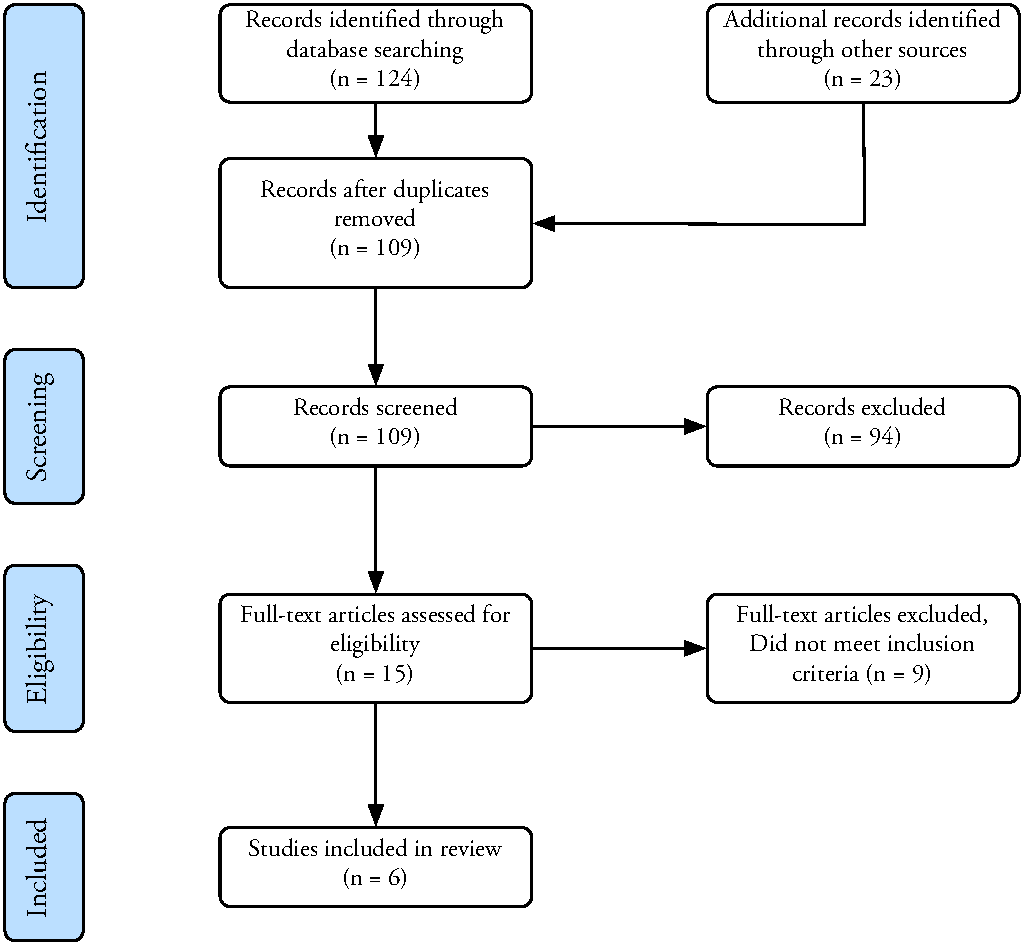
\includegraphics[keepaspectratio,width=0.9500\textwidth,height=0.75\textheight]{prismalit.pdf}
\caption{PRISMA flow diagram of search results}
\label{prismalit}
\end{figure}



\subsection{Description of studies}
\label{descriptionofstudies}

The six studies can be split into two groups, both in terms of their respective populations and methodologies. Three of the studies (Ting~\citep{ting_abstract_2009}, Selker~\citep{selker_emergency_2011} and Cantor~\citep{cantor_prehospital_2012}), included paramedics as participants and were not randomised. Instead, two were prospective diagnostic studies (Ting and Cantor) and the third, a before and after, quasi-experimental design (Selker). These studies are summarised in \autoref{tabledataextraction}.

 \renewcommand{\arraystretch}{2.0}
\newcolumntype{L}{>{\raggedright\arraybackslash}p{0.15\textwidth}}
\newcolumntype{A}{>{\raggedright\arraybackslash}p{0.24\textwidth}}
\tiny
\begin{longtable}{LAAA}
\label{tabledataextraction} \\
\caption{Summary of literature review studies (paramedic participants)} \\
\hline
\textbf{Study}&\textbf{Cantor 2012}~\citep{cantor_prehospital_2012}&\textbf{Selker 2011}~\citep{selker_emergency_2011}&\textbf{Ting 2009}~\citep{ting_abstract_2009}\\
\hline
\endfirsthead
\multicolumn{3}{l}
{\tablename\ \thetable\ -- \textit{Continued from previous page}} \\
\hline
\textbf{Study}&\textbf{Cantor 2012}&\textbf{Selker 2011}&\textbf{Ting 2009} \\
\hline
\endhead
\hline \multicolumn{4}{r}{\textit{Continued on next page}} \\
\endfoot
\hline
\endlastfoot
Population&134 consecutive patients with suspected STEMI taken for pPCI.&437 patients over three phases.&2,007 patients but only 54 patients with suspected STEMI.\\
Intervention&New protocol for primary care paramedics. Computer interpretation of 12-lead ECG (GE Marquette 12SL).&Computer interpretation using ACI-TIPI and TPI diagnostic tools. Usual computer interpretation message provided provided (GE Marquette 12SL).&Prehospital ECG protocol. Computer interpretation message provided (GE Marquette 12SL).\\
Comparison&Blinded doctor interpretation of prehospital 12-lead ECG. Final diagnosis confirmed with angiography and cardiac biomarkers.&Blinded doctor with access to patients clinical records, ECGs and cardiac biomarkers.&Diagnosis determined by angiography.\\
Outcomes&Accuracy of STEMI recognition, complications during transfer and treatment times.&Percentage of true and false positive patients identified by paramedics as having ACS or STEMI.&Accuracy of STEMI recognition by paramedics.\\
EMS system, skill level and training&Single site in Canada.  Primary care paramedics in study received 4 hours training on 12-lead ECG STEMI recognition.&11 sites throughout USA.  NAEMT certified paramedics received 4 hours training in ACS and STEMI recognition and ACI-TIPI and TPI tools.&Single site in USA.  67 NAEMT certified paramedics received 3 hours training on protocol, ECG acquisition and interpretation.\\
Results&Doctor agreed with paramedic 121\slash 134 (90\%) participants. Final diagnosis: STEMI 106\slash 134, false positive 28\slash 134. 11\slash 28 false positives could have been excluded if only computer interpretation utilised. 8 true STEMIs missed by computer interpretation.&Comparison between phase 1 and 2: STEMI identification increased from 40.8\% to 68.4\% (p$<$0.01). Retrospective analysis of ACI-TIPI and TPI gave true positive rate for STEMI as 73\%.&Prehospital recognition of STEMI: sensitivity 48.0\%, specificity 99.6\%, Positive predictive value 86.7\%, Negative predictive value 97.4\%. False negatives: 57\% due to inaccurate computer interpretation, 21\% due to cardiac arrest where no ECG recorded.\\
Notes&Primary care paramedics are equivalent to EMT-B in USA and ambulance technicians in the UK.&Training for new (to study) paramedics reduced to 1.5 hours in phase 3. Only study which utilised ACI-TIPI and TPI tools. Analysis of phases retrospective. Patients not required to have chest pain.&Only post-implementation data usable. No record of missed STEMIs not using protocol. Not clear what demographic data recorded for patients who were not in the protocol.\\
\end{longtable}
\renewcommand{\arraystretch}{1}
\normalsize 

The three remaining studies utilised doctors as participants and were randomised, utilising experimental survey designs rather than actual patient episodes (Goodacre~\citep{goodacre_computer_2001}, Massel~\citep{massel_observer_2003} and Tsai~\citep{tsai_computer_2003}). A summary of these doctor studies is provided in \autoref{tabledataextraction1}.

 \renewcommand{\arraystretch}{2.0}
\newcolumntype{P}{>{\raggedright\arraybackslash}p{0.15\textwidth}}
\newcolumntype{Q}{>{\raggedright\arraybackslash}p{0.24\textwidth}}
\tiny
\begin{longtable}{PQQQ}
\label{tabledataextraction1} \\
\caption{Summary of literature review studies (doctor participants)} \\
\hline
\textbf{Study}&\textbf{Tsai 2003}~\citep{tsai_computer_2003}&\textbf{Massel 2003}~\citep{massel_observer_2003}&\textbf{Goodacre 2001}~\citep{goodacre_computer_2001} \\
\hline
\endfirsthead
\multicolumn{4}{l}
{\tablename\ \thetable\ -- \textit{Continued from previous page}} \\
\hline
\textbf{Study}&\textbf{Tsai 2003}&\textbf{Massel 2003}&\textbf{Goodacre 2001} \\
\hline
\endhead
\hline \multicolumn{4}{r}{\textit{Continued on next page}} \\
\endfoot
\hline
\endlastfoot
Population&30 doctors (internal medical residents) in second or third year of training.&9 doctors. 3 medical residents, 3 cardiology fellows and 3 consultant cardiologists.&10 doctors, all senior house officers.\\
Intervention&23 ECGs (11 in group A, 12 in group B) with computer interpretation message.&75 ECGs with typical history, checklist and computer interpretation.&25 ECGs with computer interpretation message.\\
Comparison&23 ECGs (11 in group A, 12 in group B) with computer interpretation message hidden.&75 ECGs with atypical history, no checklist and no computer interpretation.&25 ECGs without computer interpretation message.\\
Outcomes&Interpretative accuracy of the medicine residents. Secondary outcome measure: the effect of incorrect computer interpretation.&Intra- and inter-observer variability and bias measurements.&Proportion of major errors missed in each group. Secondary outcome measure: number of completely correct ECGs, without major or minor errors.\\
Site(s)&US university department of medicine.&Single tertiary care centre in Canada.&Single emergency department in a UK teaching hospital.\\
Results&Without computer interpretation, accuracy 48.9\% (95\% CI, 45.0-52.8\%). With computer interpretation, 55.4\% (95\% CI, 51.9-58.9\%; p$<$0.0001). When the correct computer interpretation included, accuracy 68.1\% (95\% CI, 63.2-72.7\%; p$<$0.0001).  Participants wrongly agreed with incorrect computer interpretation more often when visible 67.7\% (95\% CI, 57.2-76.7\%) than when it was not 34.6\% (95\% CI, 23.8-47.3\%; p$<$0.0001).&When all doctors considered as a group, improvement in inter-observer ECG interpretation when computer message provided (p=0.0001).  Medical residents biased by computerised ECG (p$<$0.001) and less likely to recommend thrombolysis.&Major errors found in 46\slash 250 (18.4\%) ECG interpretations made by SHOs with computer interpretation visible. 56\slash 250 (22.4\%) major errors found in interpretations without computer message visible. No evidence of relationship between computer interpretation use and major errors by SHOs.\\
Notes&Computer algorithm not identified. ECGs not restricted to STEMI.&GE Marquette 12SL algorithm used. ECGs were not restricted to STEMI.&GE Marquette 12SL algorithm used. ECGs were not restricted to STEMI.\\


\end{longtable}
\renewcommand{\arraystretch}{1}
\normalsize 

\subsubsection{Paramedic studies}
\label{paramedicstudies}

The Cantor study~\citep{cantor_prehospital_2012} was a prospective diagnostic study, and enrolled 134 patients who were taken directly for pPCI at one Canadian hospital. The intervention was a newly introduced prehospital protocol, allowing primary care paramedics (PCP) to bypass local EDs in order to take patients directly to the pPCI centre. Prior to the study, PCPs received three hours training relating to 12-lead ECG interpretation.

The primary outcome was accuracy of prehospital STEMI recognition, which was compared to an experienced cardiologist who had access to the prehospital ECG, but not the angiography or cardiac biomarker results, and final diagnosis, as determined by cardiac biomarker results and angiography. Secondary outcomes included the number of complications en route and various treatment timings. In addition, computer interpretative accuracy alone, was calculated.

The Selker study~\citep{selker_emergency_2011} was a three phase, before and after quasi-experimental study, to test the use of the acute cardiac ischaemia time-insensitive predictive instrument ~\citep{selker_use_1998} and thrombolytic predictive instrument by paramedics~\citep{selker_use_2002}, to identify suitable participants for the Immediate Myocardial Metabolic Enhancement During Initial Assessment and Treatment in Emergency Care (IMMEDIATE) trial.~\citep{selker_out--hospital_2012} It was conducted in multiple sites throughout the US, with paramedics who were National Association of Emergency Medical Technicians (NAEMT) registered, and so roughly equivalent to UK paramedics. Prior to the study commencing, four hours of ECG interpretation and study tool training were provided.

The primary outcomes were proportions of patients correctly and incorrectly identified by paramedics as having an ACS, with a subsequent sub-group analysis of patients with STEMI. In addition, a retrospective analysis was conducted to determine the accuracy of the ACI-TIPI and TPI alone.

The Ting study~\citep{ting_abstract_2009} was a prospective diagnostic study conducted in the US, which collected demographic data from 2,007 patients taken by a single ambulance service to the study hospital, who were diagnosed with STEMI and underwent pPCI. The intervention was a new prehospital protocol which allowed study paramedics (NAEMT registered) to bypass the local ED and take patients directly to the study hospital's cardiac catheter lab. Prior to the start of the study, paramedics received three hours training, including familiarisation with the study protocol and 12-lead ECG acquisition and interpretation.

The primary outcome was accuracy of paramedic recognition of STEMI, which was compared to final hospital discharge diagnosis determined by ECG findings, angiography and successful reperfusion with pPCI. 

\subsubsection{Doctor studies}
\label{doctorstudies}

The Tsai study~\citep{tsai_computer_2003} was a randomised crossover controlled trial with 30 internal medicine residents from a single US university medical centre, who were in their second or third year of training. The participants were stratified according to year of training and then randomly allocated into one of two groups, which determined in which order the ECGs with computer interpretation would be viewed. Group A contained 11 ECGs and group B, 12, making a total of 23 ECGs. The study took place over a five-month period, with the ECG interpretation being conducted as a one-hour, supervised session.

The primary outcome was interpretative accuracy of the medicine residents, with a secondary outcome of the effect of incorrect computer interpretation on the participant's interpretations which were incorrect.

The Massel study~\citep{massel_observer_2003} was a two-by-two-by-two factorial randomised control trial (RCT) with nine participants from a single tertiary teaching hospital in Canada. There were three doctors from each of the following grades:

\begin{itemize}
\item Medical resident

\item Cardiology fellow

\item Consultant cardiologist.

\end{itemize}

The participants reviewed 75 ECGs, selected from the coronary care unit (CCU) and hospital patients by the researchers. Due to the factorial design, they were required to review the ECGs eight times over an eight-month period.

The primary outcome was the reliability and accuracy of ECG interpretation and the effect of three contributing factors (clinical history, a checklist developed as part of the study and computer interpretation).

The Goodacre study~\citep{goodacre_computer_2001} was an RCT with 10 participants, all junior doctors, working at a single UK teaching hospital emergency department. They reviewed 50 ECGs (half with the computer interpretation message visible and half without) at a single sitting, and under examination conditions.

The primary outcome was the proportion of major errors missed in each group, with a secondary outcome measure of the number of completely correct ECG interpretations (i.e. those without major and minor errors specified by the study design). 

\subsection{Methodological quality}
\label{methodologicalquality}

\subsubsection{Validity}
\label{validity}

All six studies had a clear research question, which conformed to the population, intervention, comparison, outcome (PICO) model. Only one of the studies~\citep{goodacre_computer_2001} was conducted in the UK, with the remainder conducted in North America (three from the US~\citep{tsai_computer_2003,ting_abstract_2009,selker_emergency_2011} and two from Canada~\citep{massel_observer_2003,cantor_prehospital_2012}). There was a clear distinction between the studies involving paramedics, which included patients with suspected acute coronary syndromes (ACS), and those with doctors as participants, which utilised previously obtained ECGs.

The eligibility criteria in the paramedic studies were typically two-fold, since both para-medics and patients were required. Skill levels were specified, with paramedics in the Selker and Ting studies having comparable qualifications to that of UK paramedics (i.e. NAEMT paramedic registration), whereas the Cantor study utilised Canadian primary care paramedics, equivalent to UK ambulance technicians, the tier below paramedics. The patients in the paramedics studies also had slightly differing eligibility criteria, with Selker and Cantor not stipulating an age limit, but specifying a requirement for patients to present with signs and symptoms of ACS, whereas the Ting study only considered the ECG criteria, and patients were only eligible for entry into the study if there was agreement between paramedic and computer interpretation. The Selker and Cantor studies also allowed local protocols and the paramedic's judgement to override the study criteria. 

A key omission in determining the accuracy of paramedic's interpretation in all studies, was the omission of patients who did not undergo pPCI at the study hospital, or, in the case of the Selker study, were not identified as having an ACS and so not enrolled. In addition, none of the studies compared paramedics’ diagnoses alone. Therefore, without the benefit of computer interpretation, differentiating the effect that paramedic and computer interpretations had on the accuracy of diagnosis is difficult to determine, even when the computer interpretation accuracy rates were reported separately.

The doctor studies all involved junior doctors (defined as being 2--3 years post-graduation), although Massel also included middle and senior grades. No information was provided about how the participants were recruited, but the randomisation strategy was clearly laid out in all studies, although none included a consolidated standards of reporting trials (CONSORT) flow diagram~\citep{schulz_consort_2010}. All participants were accounted for and none were lost to follow-up.

In the paramedic studies, it was apparent that some patients did not receive the diagnostic test and\slash or had the reference standard applied. Nine patients in the Ting study did not have a prehospital 12-lead ECG, but were subsequently taken for pPCI and included in the results as false negatives. No two-by-two table was included, although it is possible to calculate this from the sensitivity, specificity, negative and positive predictive values provided. Almost 3\% of patients in the Selker study did not have an ACI-TIPI score calculated, leading to a risk of verification bias~\citep{lijmer_empirical_1999}. A two-by-two table was not provided in the results, as only the test positive results were included. There was no missing data in the Cantor study, although one patient did not receive the reference standard test (pPCI) since the patient was considered to be a false positive and so not appropriate for pPCI.

The reference standard for the doctor studies were senior cardiologists or ED consultants, who independently reviewed the study ECGs prior to the study commencing, and who were blinded to the computer interpretation result. Their responses were collated and any disagreements were resolved by discussion. When assessing the participants' responses, only the Tsai study made it clear that the marker was blinded to the participant identity and computer interpretation message. However, the marking in this study was conducted by only one researcher. The Goldacre study blinded the assessors to the computer report, but it was not clear whether they were blinded to the participant identity. However, in contrast to the Tsai study, both ED consultants independently reviewed the participants' results and their agreement was measured by the calculation of the $  \kappa  $ statistic, with disagreements resolved by discussion. The Massel study provides no information about whether the researchers were blinded to the participant identity or the presence of the computer interpretation message, which could be a source of review bias~\citep{whiting_sources_2004}. However, the participants were blinded to their previous answers and those of fellow participants. 

All three paramedic studies used angiography and cardiac biomarkers as the reference standard for diagnosis. In addition, two of the paramedic studies (Selker and Cantor), also used a doctor with access to the patients' notes, but blinded to the paramedic's study results as an additional reference standard. The Ting study did not specify whether the research staff accessing the patients' notes were blinded.

Four of the studies utilised the GE Marquette 12SL algorithm, with the Tsai and Massel studies failing to identify the algorithm used. In addition, the Selker study also utilised two additional novel algorithms (ACI-TIPI and TPI) in the latter phases of their study.

The study procedures were clearly outlined in all studies, although in the case of the Ting study (published as a conference abstract), it was necessary to obtain a further article to review the protocol, after the lead author failed to respond to direct communication~\citep{nestler_impact_2011}. Eligibility criteria were provided for all of the paramedic studies, but little explanation was provided in the doctor studies. Baseline characteristics of patients were provided in two of the paramedics studies, with only Cantor failing to provide any demographic or co-morbidity information, making assessment of spectrum bias impossible~\citep{whiting_sources_2004}. All of the doctor studies provided current job role and years since graduation, but only Massel provided additional data about average ECG interpretations conducted by the participant per week. This was lacking in the Goodacre and Tsai studies, making it difficult to determine whether control and intervention groups were equivalent. The Tsai study describes the design as a matched pairs crossover design, but the only matching that appears to have been conducted was years since graduation. In addition, a single participant did not see the same ECG twice, once with and without the computer interpretation, but instead saw an equivalent set of ECGs for each phase. Massel used a crossover design, and participants saw the same ECG on multiple occasions, both with and without the computer interpretation. These issues aside, all of the doctor studies did treat the intervention and control arms of the studies in the same way, except for applying the intervention.

\subsubsection{Results}
\label{results}

While all three of the paramedic studies provided information about the accuracy of computer interpretation alone, it was not possible to determine the accuracy of the paramedics alone, since all were exposed to the computer interpretation when making a diagnosis. The doctor studies in comparison, thanks to their randomised control trial design, provide responses with and without the computer interpretation.

In the Cantor study, paramedics identified 134 patients as suspected STEMI and were correct in 106 (79\%) of cases. If the diagnosis had been made by computer interpretation alone, 98\slash 106 (92\%) of patients with STEMI would have been correctly identified, correctly excluding a further 11\slash 28 (39\%) of the false positives.

The three phase design of the Selker study makes analysis of the results rather more complicated. All three phases provided paramedics with computer interpretation, however in the latter phases, the criteria were amended to require an ACI-TIPI prediction of 75\% or more, or a TPI prediction of STEMI. Despite this, paramedics were still able to activate their local pPCI pathway if the local emergency medical service (EMS) protocol eligibility criteria was met. The study found a statistically significant increase in the percentage of patients with STEMI between phases 1 and 2, rising from 40.8\% to 68.4\%. However, since the study also included patients with ACS and not just STEMI, it makes direct comparison with the other paramedic studies difficult. A retrospective analysis by the researchers explored the ACI-TIPI and TPI across all three phases and found that, in cases of confirmed ACS, the computer correctly identified 226\slash 284 (80\%) of patients, compared with paramedics with computer interpretation, who correctly identified 296\slash 437 (68\%).

The Ting study was the only one to provide sufficient information to construct a two-by-two table. In addition, although study protocol required that paramedic and computer interpretation had to agree in order for the patient to be considered for direct admission to the cardiac catheter unit, patients who were taken to the study hospital and who had a final diagnosis of STEMI were also included. This made it possible to identify occurrences when the paramedic and computer disagreed. Paramedics agreed with the computer interpretation in 26\slash 54 (48.1\%) of STEMI cases. If only the paramedic's interpretation had been required, correct recognition would have increased to 43\slash 54 (79.6\%).

The Tsai study reported correct and incorrect results for computer interpretation alone, participants alone, and participants with the computer message. However, only 18\slash 54 of the study ECGs could be considered to be STEMI or STEMI-mimic in morphology, which limits the results' applicability to the RESPECT study. Results were reported as average (presumably means, although this was not stated) values. In the sub-category of correct computer interpretation, 53\% of participants correctly interpreted the ECG without the computer message, with a statistically significant increase to 68\%, when it was visible. However, when the computer interpretation was incorrect, participants were incorrect 35\% of the time when the message was hidden, rising to a statistically significant 68\% when the incorrect message was shown.

The Massel study utilised a two-by-two-by-two factorial design, requiring participants to view ECGs on four separate occasions with and without the computer interpretation, and with differing combinations clinical history and the presence (or absence) of a checklist. Results were reported using inter- and intra-class reliability measures ($  \kappa $ statistics) and tendencies of bias. Mean overcalls and undercalls for thrombolysis eligibility were also reported, including 95\% confidence intervals. Only the medical residents had statistically significant effects caused by the presence of the computer interpretation message. They were biased by the computer interpretation and more likely to undercall thrombolysis (the mean undercall rose from 5.4\% to 8.5\% in the presence of the computer interpretation message). In the sub-group of ECGs which were accompanied by a typical history of AMI, medical residents were more likely to change their decision in favour of thrombolysis if the computer interpretation was provided.

The Goodacre study consisted of 10 junior ED doctors who each interpreted 50 ECGs, 25 with a computer interpretation and 25 without. As with the Massel study, ECGs were not exclusively limited to STEMI and the breakdown of ECG findings was not reported. Interpretations were classified into three categories: completely correct, major errors and minor errors. The criteria for major errors did include ST-segment elevation of $>$1mm. Results were reported as proportions, with confidence intervals and p-values provided. Overall, the computer interpretation messages had no statistically significant effect on the participants. Major errors occurred in 46\slash 250 (18\%) of interpretations with the computer message, which rose to 56\slash 250 (22\%) without (p=0.13). Participants correctly interpreted 104\slash 250 (42\%) ECGs with the computer message and 91\slash 250 (36.4\%) without (p=0.15).

Only the Goodacre study provided a power calculation to justify the sample size chosen, but this did not account for the clustering of data in the study. In fact, none of the studies took clustering into account in the analysis of data. The Tsai study did acknowledge the multi-level nature of the data, but assumed that this would not have any effect. This is unwise, since not accounting for clustering leads to smaller standard errors (and confidence intervals), increasing the likelihood that chance findings will be considered to be statistically significant~\citep{bland_statistics_1997}. 

\subsubsection{Context}
\label{context}

The literature review has highlighted the absence of studies directly examining the effect of computer interpretation messages on paramedic's recognition of STEMI. The paramedic studies identified in the review do have a clinically relevant context, but the lack of results of paramedic interpretation alone, makes it impossible to isolate the effect of the computer interpretation. The studies do suggest that computer interpretation has an effect, but not whether this is clinically significant.

The doctor studies are able to determine the effect of computer interpretation alone, however, this is a distinctly different population to paramedics, and the results of the studies lack generalisability, due to the small numbers of participants. In addition, ECG interpretation was not limited to STEMI or STEMI-mimics in two of the studies (Goodacre and Tsai), further reducing their applicability to the research question. This is compounded by the failure to account for the clustering effects of the data.

Only one of the studies was based in the UK (Goodacre, a doctor study), and one of the paramedic studies was conducted with paramedics who have a skill equivalent of ambulance technicians in the UK.

In conclusion, the methodology of the doctor studies provides a good indication about how this research question could be answered if the correct population is identified. Thus, a sufficiently powered randomised crossover trial with UK paramedics would provide an sound basis on which to answer the research question for this dissertation.
